\documentclass[11pt,a4paper]{article}
\usepackage[top=2cm, bottom=2.3cm, left=1.8cm, right=1.8cm, headsep=0.8cm]{geometry}
\usepackage{amsmath,amssymb,amsfonts}
\usepackage{graphicx}
\graphicspath{{images/}{public/exam-images/SohanMock/}{./}}
\usepackage{enumitem}
\usepackage{fancyhdr}
\usepackage[table]{xcolor}
\usepackage{tcolorbox}
\tcbuselibrary{breakable,skins}
\usepackage{tabularx}
\usepackage{multicol}

% High-Contrast Modern Color Palette
\definecolor{primaryDark}{RGB}{12, 32, 84}       % Midnight Navy (Deep)
\definecolor{primaryBlue}{RGB}{18, 72, 160}      % Solid Royal Blue
\definecolor{goldAccent}{RGB}{255, 215, 0}       % Gold highlight
\definecolor{l1Green}{RGB}{14, 120, 62}          % Vivid Forest Green
\definecolor{l2Amber}{RGB}{205, 80, 0}           % Rich Amber / Orange
\definecolor{l3Crimson}{RGB}{180, 20, 20}        % Deep Crimson Red
\definecolor{formulaBg}{RGB}{255, 252, 235}      % Warm Cream-Gold
\definecolor{formulaBorder}{RGB}{220, 160, 30}   % Gold Border
\definecolor{cardBg}{RGB}{250, 252, 255}         % Clean Crisp Card Background
\definecolor{cardBorder}{RGB}{130, 170, 220}     % Sharp Steel Blue Border
\definecolor{tableStripe}{RGB}{242, 246, 252}    % Alternating Table Row
\definecolor{tableDarkHeader}{RGB}{12, 32, 84}   % Dark Table Header
\definecolor{darkCharcoal}{RGB}{25, 25, 25}      % High-contrast body text

% Page styling (Guaranteed Collision-Free Header)
\pagestyle{fancy}
\fancyhf{}
\setlength{\headheight}{16pt}
\fancyhead[L]{\small\textsf{\textbf{\textcolor{primaryDark}{Sohan Mocks Series}} $\vert$ \textbf{\textcolor{primaryBlue}{Physics: Gravitation (Very Hard)}}}}
\fancyhead[R]{\small\textsf{\textbf{\textcolor{l3Crimson}{Max Marks: 100 $\vert$ 60 Mins}}}}
\fancyfoot[C]{\textbf{\textsf{\thepage}}}
\renewcommand{\headrulewidth}{0.8pt}
\renewcommand{\footrulewidth}{0.4pt}

% Custom High-Contrast tcolorboxes
\tcbset{
  dayheader/.style={
    colback=primaryDark,
    coltext=white,
    boxrule=0pt,
    arc=3mm,
    left=14pt, right=14pt, top=10pt, bottom=10pt
  },
  sectionbanner/.style={
    colback=primaryBlue,
    coltext=white,
    boxrule=0pt,
    arc=2mm,
    left=10pt, right=10pt, top=6pt, bottom=6pt
  },
  solbox/.style={
    enhanced,
    breakable,
    colback=cardBg,
    colframe=cardBorder,
    boxrule=1.0pt,
    arc=2mm,
    left=10pt, right=10pt, top=7pt, bottom=7pt
  }
}

\begin{document}

% ==================== TEST HEADER BANNER ====================
\begin{tcolorbox}[dayheader]
\begin{center}
  {\Large \textbf{\textsf{\textcolor{goldAccent}{SOHAN MOCKS ADVANCED TEST SERIES}}}}\\[3pt]
  {\LARGE \textbf{\textsf{TOPICAL SPECIAL: GRAVITATION (VERY HARD PAPER)}}}\\[5pt]
  {\normalsize \textbf{\textsf{Core Domains:}} Kepler Orbits $\vert$ Variable Density Field $\vert$ Cavity Superposition $\vert$ Tunnel SHM $\vert$ Hohmann Transfer $\vert$ Self-Energy}\\[3pt]
  {\footnotesize \textbf{Exam Pattern:} 25 Questions (20 MCQs $+4/-1$ + 5 Numerical $+4/0$) \quad $\vert$ \quad \textbf{Time:} 60 Minutes \quad $\vert$ \quad \textbf{Max Marks:} 100}
\end{center}
\end{tcolorbox}

\vspace{6pt}

% ==================== SECTION I: SINGLE CORRECT CHOICE ====================
\begin{tcolorbox}[sectionbanner]
  {\large \textbf{\textsf{SECTION I: SINGLE CORRECT CHOICE TYPE (Q01 -- Q20)}}} \hfill {\small \textbf{Marking: $+4$ / $-1$}}
\end{tcolorbox}
\vspace{4pt}

\begin{enumerate}[label=\textbf{\arabic*.},leftmargin=18pt,itemsep=10pt]

  \item A satellite of mass $m$ is orbiting Earth (mass $M$, radius $R$) in an eccentric elliptical orbit, as shown in the accompanying diagram. The perigee distance from the center of Earth is $r_p = 2R$ and the apogee distance is $r_a = 6R$. Using the conservation of angular momentum and mechanical energy, find the speed of the satellite at the perigee ($v_p$).
  \begin{center}
    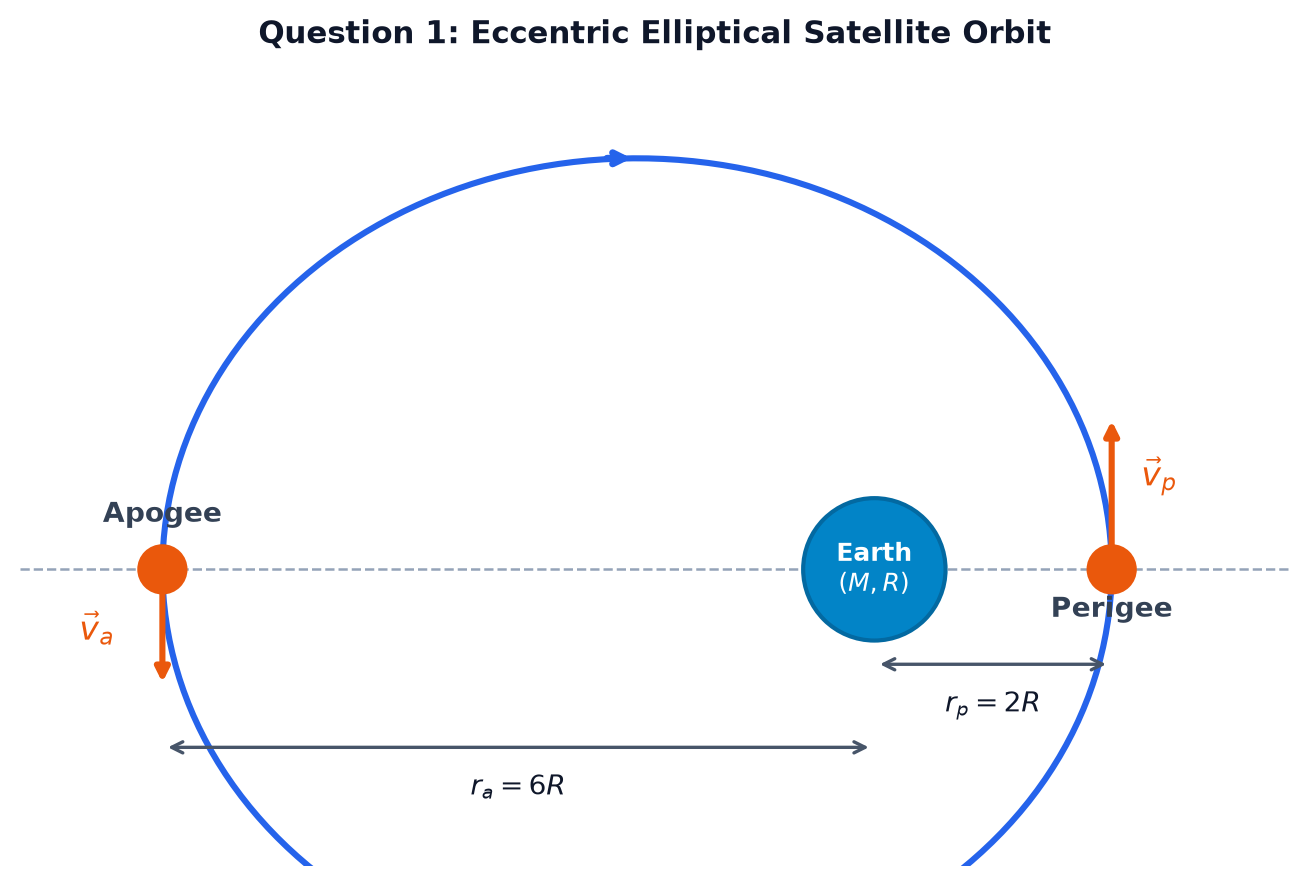
\includegraphics[width=0.40\textwidth]{images/sohan_grav_q01_ellipse.png}
  \end{center}
  \begin{multicols}{4}
    \begin{enumerate}[label=(\Alph*)]
      \item $\sqrt{\dfrac{GM}{2R}}$
      \item $\dfrac{\sqrt{3}}{2}\sqrt{\dfrac{GM}{R}}$
      \item $\sqrt{\dfrac{3GM}{2R}}$
      \item $\sqrt{\dfrac{2GM}{3R}}$
    \end{enumerate}
  \end{multicols}

  \item A solid sphere of radius $R$ and uniform mass density $\rho$ has a spherical cavity of radius $R/2$ scooped out of it, as illustrated in the figure. The center of the cavity is displaced by a vector $\vec{d}$ from the center of the sphere ($|\vec{d}| = R/2$). What is the gravitational field $\vec{g}$ at any arbitrary point inside the cavity?
  \begin{center}
    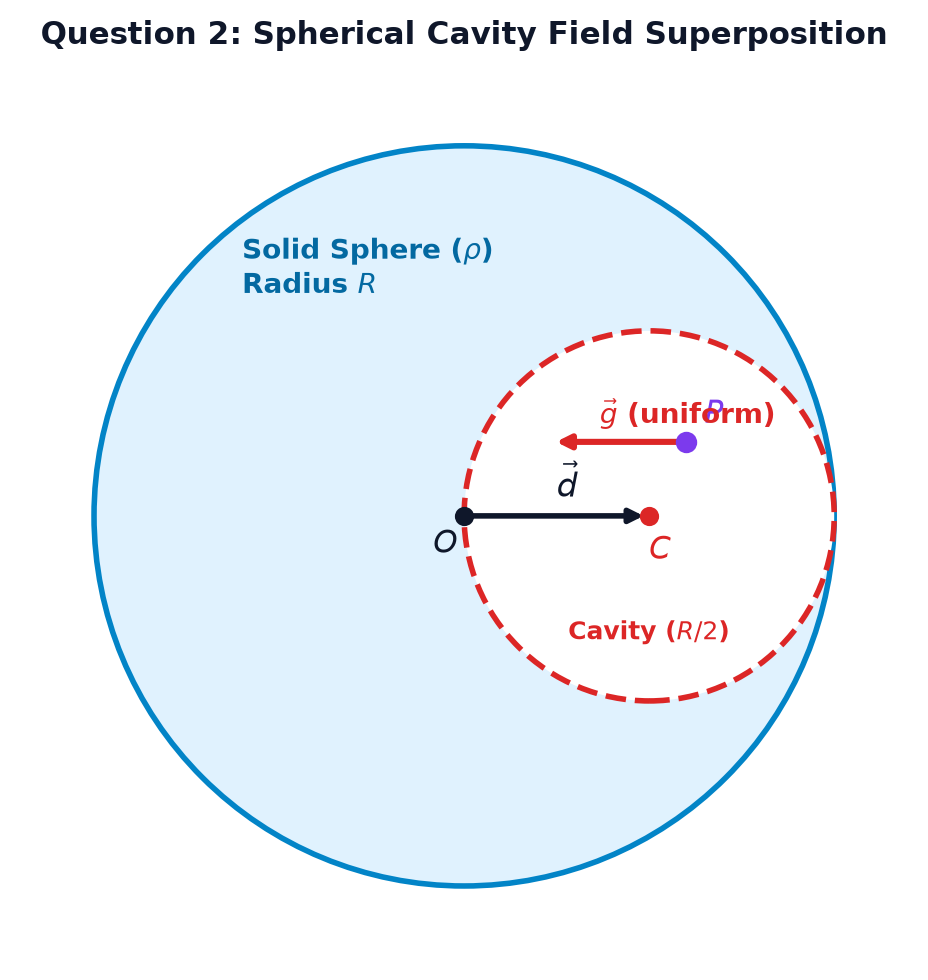
\includegraphics[width=0.34\textwidth]{images/sohan_grav_q02_cavity.png}
  \end{center}
  \begin{multicols}{2}
    \begin{enumerate}[label=(\Alph*)]
      \item Variable, depending on the position vector of the point
      \item Strictly zero throughout the cavity
      \item Uniform with magnitude $\dfrac{2}{3}\pi G \rho R$ directed opposite to $\vec{d}$
      \item Uniform with magnitude $\dfrac{4}{3}\pi G \rho R$ directed along $\vec{d}$
    \end{enumerate}
  \end{multicols}

  \item A smooth straight tunnel is dug through Earth (mass $M$, radius $R$, uniform density $\rho$) along a chord situated at a perpendicular distance $d = R/2$ from the Earth's center, as depicted in the figure. A small particle of mass $m$ is released from rest inside the tunnel. Which of the following statements is INCORRECT?
  \begin{center}
    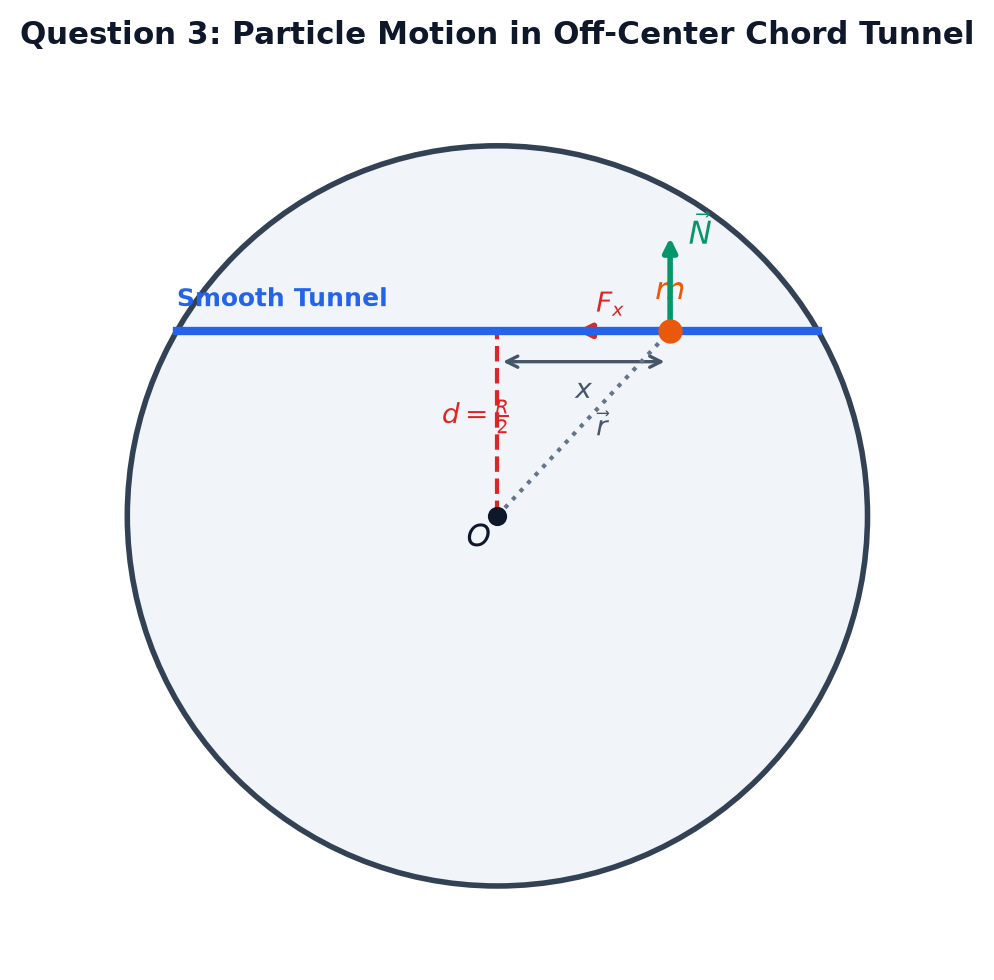
\includegraphics[width=0.34\textwidth]{images/sohan_grav_q03_tunnel.png}
  \end{center}
  \begin{multicols}{2}
    \begin{enumerate}[label=(\Alph*)]
      \item The particle executes simple harmonic motion along the tunnel
      \item The period of oscillation is $T = 2\pi\sqrt{\dfrac{R}{g}}$
      \item The normal force exerted by the tunnel wall on the particle varies with time as $N(t) = mg\cos(\omega t)$
      \item The normal force exerted by the tunnel wall on the particle is constant and equal to $\dfrac{mg}{2}$
    \end{enumerate}
  \end{multicols}

  \item A meteorite of mass $m$ approaches a planet of mass $M$ and radius $R$ from an infinite distance with an initial asymptotic speed $v_0$ and an impact parameter $b$. For the meteorite to collide with or graze the planet's surface, the impact parameter $b$ must satisfy:
  \begin{multicols}{2}
    \begin{enumerate}[label=(\Alph*)]
      \item $b \le R\sqrt{1 + \dfrac{2GM}{R v_0^2}}$
      \item $b \le R\left(1 + \dfrac{2GM}{R v_0^2}\right)$
      \item $b \le R\sqrt{\dfrac{2GM}{R v_0^2}}$
      \item $b \le \dfrac{R v_0}{\sqrt{2GM/R}}$
    \end{enumerate}
  \end{multicols}

  \item Three identical stars, each of mass $M$, move in circular orbits around their common center of mass $G$ under their mutual gravitational attraction, as depicted in the figure. Throughout the motion, they always remain at the vertices of an equilateral triangle of side $R$. The orbital speed $v$ and orbital period $T$ of each star are:
  \begin{center}
    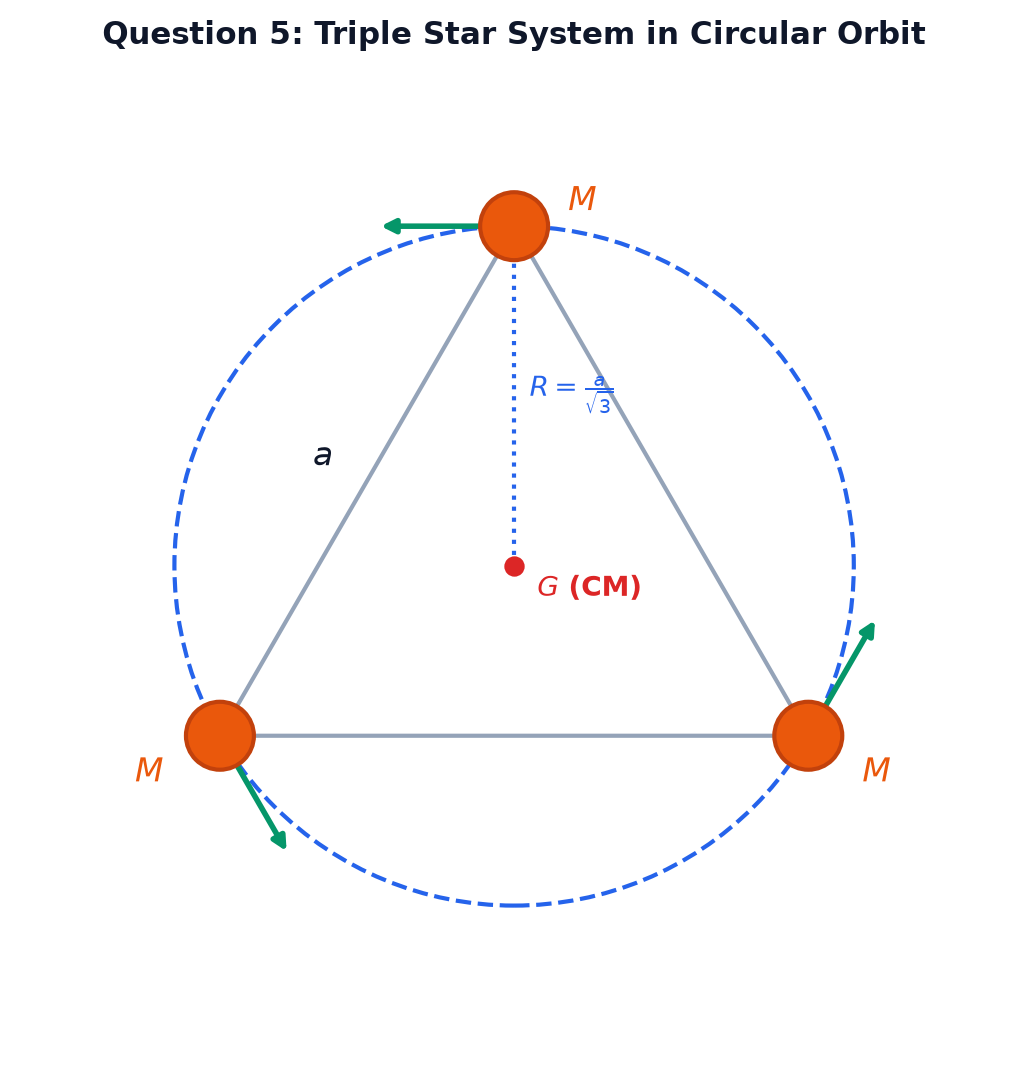
\includegraphics[width=0.34\textwidth]{images/sohan_grav_q05_triplestar.png}
  \end{center}
  \begin{multicols}{2}
    \begin{enumerate}[label=(\Alph*)]
      \item $v = \sqrt{\dfrac{GM}{R\sqrt{3}}}, \quad T = 2\pi\sqrt{\dfrac{R^3\sqrt{3}}{GM}}$
      \item $v = \sqrt{\dfrac{3GM}{R}}, \quad T = 2\pi\sqrt{\dfrac{R^3}{3GM}}$
      \item $v = \sqrt{\dfrac{GM}{3R}}, \quad T = 2\pi\sqrt{\dfrac{3R^3}{GM}}$
      \item $v = \sqrt{\dfrac{2GM}{R\sqrt{3}}}, \quad T = 2\pi\sqrt{\dfrac{R^3}{2GM}}$
    \end{enumerate}
  \end{multicols}

  \item A spherically symmetric planet of radius $R$ has a volume mass density that varies with radial distance $r$ from the center as $\rho(r) = \rho_0 \left(1 - \dfrac{r}{R}\right)$ for $r \le R$, where $\rho_0$ is the central density. The radial distance $r$ from the center where the gravitational field intensity is maximum is:
  \begin{multicols}{4}
    \begin{enumerate}[label=(\Alph*)]
      \item $\dfrac{R}{2}$
      \item $\dfrac{2R}{3}$
      \item $\dfrac{3R}{4}$
      \item $\dfrac{R}{3}$
    \end{enumerate}
  \end{multicols}

  \item If the escape velocity of a body from the surface of a uniform solid sphere of mass $M$ and radius $R$ is $v_e$, the minimum velocity with which a body must be projected from the center of the sphere to escape its gravitational pull to infinity is:
  \begin{multicols}{4}
    \begin{enumerate}[label=(\Alph*)]
      \item $\sqrt{2}\,v_e$
      \item $\sqrt{1.5}\,v_e$
      \item $2\,v_e$
      \item $\sqrt{3}\,v_e$
    \end{enumerate}
  \end{multicols}

  \item A spacecraft is orbiting in a circular parking orbit of radius $r_1 = R$ around Earth (mass $M$). To transfer the spacecraft to a higher circular orbit of radius $r_2 = 4R$, it is injected into an elliptical Hohmann transfer orbit. The velocity increment $\Delta v_1$ required at the first perigee firing is:
  \begin{multicols}{2}
    \begin{enumerate}[label=(\Alph*)]
      \item $\left(\sqrt{\dfrac{8}{5}} - 1\right)\sqrt{\dfrac{GM}{R}}$
      \item $\left(\sqrt{\dfrac{5}{2}} - 1\right)\sqrt{\dfrac{GM}{R}}$
      \item $\left(\sqrt{2} - 1\right)\sqrt{\dfrac{GM}{R}}$
      \item $\left(1 - \sqrt{\dfrac{2}{5}}\right)\sqrt{\dfrac{GM}{R}}$
    \end{enumerate}
  \end{multicols}

  \item The total self-gravitational potential energy of a uniform solid planet of mass $M$ and radius $R$ is $U = -\dfrac{3GM^2}{5R}$. How much mechanical work must be done by an external agent to completely disperse the material of the planet into infinitely separated dust particles?
  \begin{multicols}{4}
    \begin{enumerate}[label=(\Alph*)]
      \item $\dfrac{GM^2}{2R}$
      \item $\dfrac{3GM^2}{5R}$
      \item $\dfrac{3GM^2}{10R}$
      \item $\dfrac{6GM^2}{5R}$
    \end{enumerate}
  \end{multicols}

  \item A thin uniform hemispherical shell of mass $M$ and radius $R$ is placed such that its circular rim lies in the $xy$-plane with its center at the origin $O$. The magnitude of the gravitational field intensity at the origin $O$ is:
  \begin{multicols}{4}
    \begin{enumerate}[label=(\Alph*)]
      \item $\dfrac{GM}{2R^2}$
      \item $\dfrac{GM}{R^2}$
      \item $\dfrac{2GM}{\pi R^2}$
      \item $\dfrac{GM}{4R^2}$
    \end{enumerate}
  \end{multicols}

  \item A thin uniform circular ring has mass $M$ and radius $R$. Gravitational field intensity $g(x)$ is measured at an axial point $P$ at a distance $x$ from the center of the ring, as shown in the diagram. At what distance $x$ along the axis from the center of the ring is the magnitude of the gravitational field maximum, and what is this maximum value?
  \begin{center}
    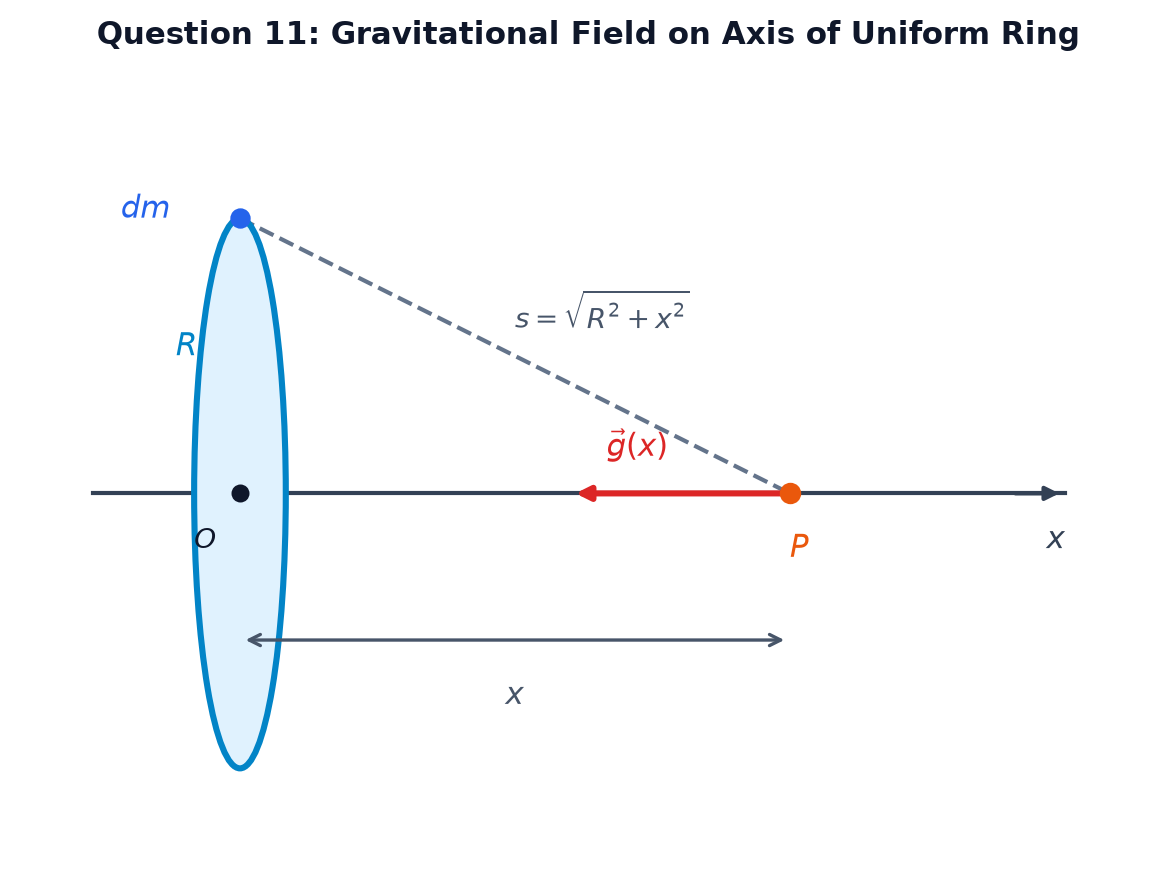
\includegraphics[width=0.38\textwidth]{images/sohan_grav_q11_axialring.png}
  \end{center}
  \begin{multicols}{2}
    \begin{enumerate}[label=(\Alph*)]
      \item $x = \dfrac{R}{\sqrt{2}}, \quad g_{\max} = \dfrac{2GM}{3\sqrt{3}R^2}$
      \item $x = R, \quad g_{\max} = \dfrac{GM}{2\sqrt{2}R^2}$
      \item $x = \dfrac{R}{2}, \quad g_{\max} = \dfrac{4GM}{5\sqrt{5}R^2}$
      \item $x = R\sqrt{2}, \quad g_{\max} = \dfrac{GM}{3\sqrt{3}R^2}$
    \end{enumerate}
  \end{multicols}

  \item Taking Earth as a sphere of radius $R$ rotating with angular velocity $\omega$ about its polar axis, the apparent acceleration due to gravity at latitude $\lambda$ is $g' = g - \omega^2 R\cos^2\lambda$. The angle $\alpha$ by which a plumb line deviates from the true radial line passing through Earth's center attains its maximum value at a latitude of:
  \begin{multicols}{4}
    \begin{enumerate}[label=(\Alph*)]
      \item $\lambda = 0^\circ$ (Equator)
      \item $\lambda = 90^\circ$ (Poles)
      \item $\lambda = 45^\circ$
      \item $\lambda = 60^\circ$
    \end{enumerate}
  \end{multicols}

  \item Two solid spherical bodies of masses $M$ and $5M$ and radii $R$ and $2R$ respectively are released from rest in deep space when their centers are separated by a distance $12R$. If they move only under mutual gravitational attraction, the distance traveled by the smaller body of mass $M$ before collision is:
  \begin{multicols}{4}
    \begin{enumerate}[label=(\Alph*)]
      \item $7.5 R$
      \item $4.5 R$
      \item $9.0 R$
      \item $6.0 R$
    \end{enumerate}
  \end{multicols}

  \item A rocket is launched from Earth's surface with an initial velocity $v = \sqrt{5}\,v_e$, where $v_e = \sqrt{2gR}$ is the escape velocity from Earth. Far away from Earth in interstellar space, its asymptotic speed $v_\infty$ will be:
  \begin{multicols}{4}
    \begin{enumerate}[label=(\Alph*)]
      \item $v_e$
      \item $2 v_e$
      \item $\sqrt{5}\,v_e$
      \item $4 v_e$
    \end{enumerate}
  \end{multicols}

  \item A small satellite moves in a circular orbit grazing the surface of a spherical planet of uniform density $\rho$ and radius $R$. The orbital period $T$ of the satellite:
  \begin{multicols}{2}
    \begin{enumerate}[label=(\Alph*)]
      \item Is proportional to $\sqrt{R}$
      \item Is proportional to $R$
      \item Depends only on density $\rho$ as $T = \sqrt{\dfrac{3\pi}{G\rho}}$ and is independent of $R$
      \item Is proportional to $1/\sqrt{R}$
    \end{enumerate}
  \end{multicols}

  \item Two thin concentric spherical shells have masses $M_1$ and $M_2$ and radii $R_1$ and $R_2$ ($R_1 < R_2$). A point mass $m$ is moved slowly by an external agent from the surface of the inner shell ($r = R_1$) to the surface of the outer shell ($r = R_2$). The work done by the external agent is:
  \begin{multicols}{2}
    \begin{enumerate}[label=(\Alph*)]
      \item $G M_1 m \left(\dfrac{1}{R_1} - \dfrac{1}{R_2}\right)$
      \item $G (M_1 + M_2) m \left(\dfrac{1}{R_1} - \dfrac{1}{R_2}\right)$
      \item $G M_2 m \left(\dfrac{1}{R_1} - \dfrac{1}{R_2}\right)$
      \item $\text{Zero}$
    \end{enumerate}
  \end{multicols}

  \item A celestial body moves in an elliptical orbit of eccentricity $e$ around a massive star. The ratio of its linear speed at perihelion $v_p$ to its linear speed at aphelion $v_a$ is:
  \begin{multicols}{4}
    \begin{enumerate}[label=(\Alph*)]
      \item $\dfrac{1+e}{1-e}$
      \item $\sqrt{\dfrac{1+e}{1-e}}$
      \item $\left(\dfrac{1+e}{1-e}\right)^2$
      \item $\dfrac{1}{1-e^2}$
    \end{enumerate}
  \end{multicols}

  \item A dumbbell consisting of two equal point masses $m$ connected by a light rigid rod of length $2\ell$ is oriented radially at a distance $r \gg \ell$ from a star of mass $M$. The differential gravitational force (tidal tension) experienced by the rod between the two masses is:
  \begin{multicols}{4}
    \begin{enumerate}[label=(\Alph*)]
      \item $\dfrac{2GMm\ell}{r^3}$
      \item $\dfrac{GMm\ell}{r^3}$
      \item $\dfrac{4GMm\ell}{r^3}$
      \item $\dfrac{GMm}{r^2}$
    \end{enumerate}
  \end{multicols}

  \item A spherical cloud of interstellar gas has mass $M$, radius $R$, and volume density $\rho(r) = \dfrac{C}{r}$ for $r \le R$, where $C$ is a positive constant. The gravitational field intensity inside the cloud at distance $r$ from the center is:
  \begin{multicols}{4}
    \begin{enumerate}[label=(\Alph*)]
      \item Independent of $r$ and constant
      \item Proportional to $r$
      \item Proportional to $1/r$
      \item Proportional to $r^2$
    \end{enumerate}
  \end{multicols}

  \item A uniform thin ring of mass $m$ and radius $R$ is placed directly above a uniform solid sphere of mass $M$ and equal radius $R$ such that the center of the ring is at a vertical height $h = R$ directly above the center of the sphere (see figure). The gravitational force of attraction between the ring and the sphere is:
  \begin{center}
    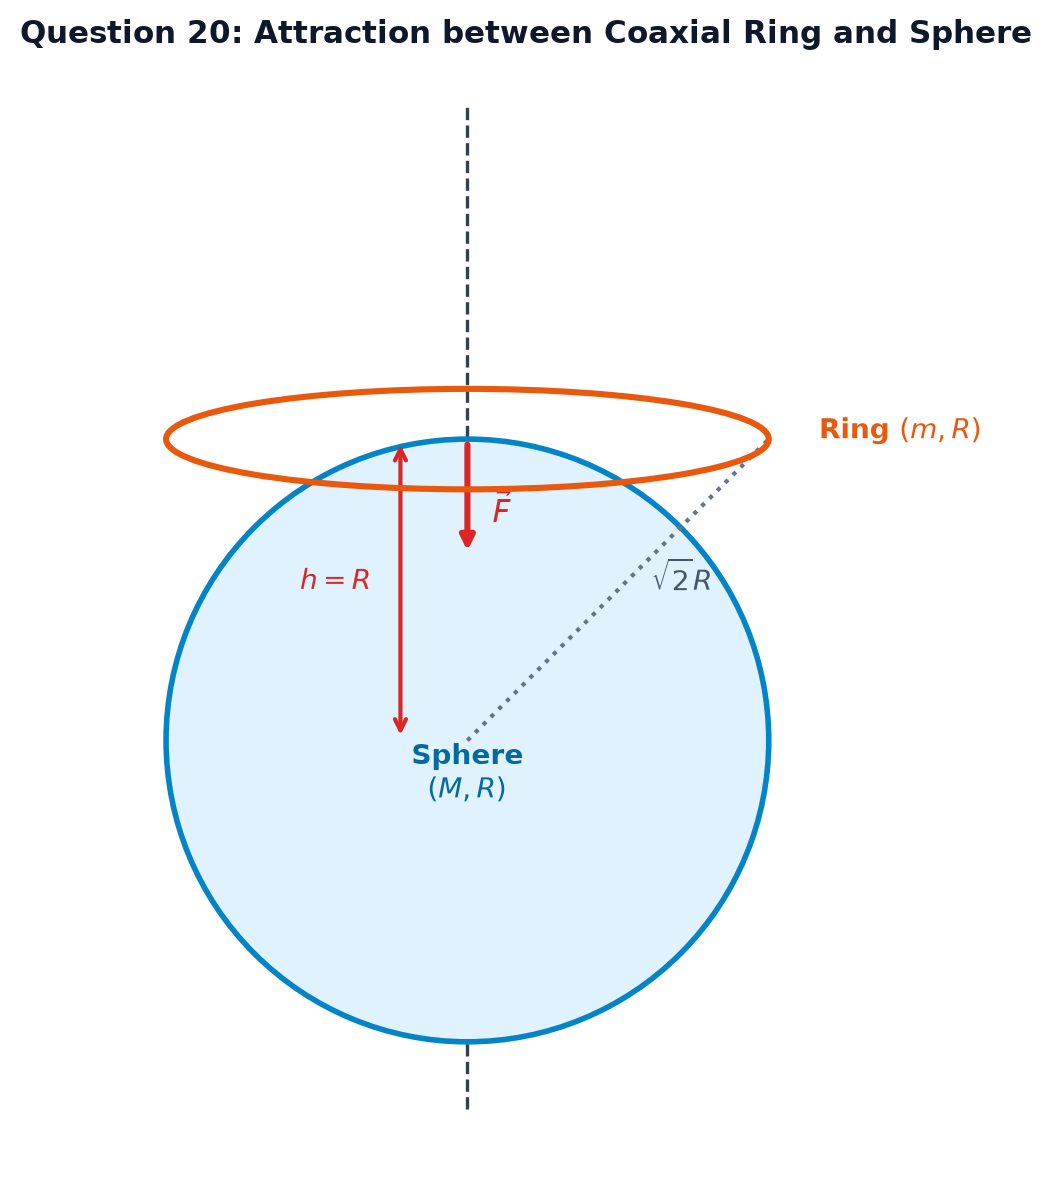
\includegraphics[width=0.32\textwidth]{images/sohan_grav_q20_ring_sphere.png}
  \end{center}
  \begin{multicols}{4}
    \begin{enumerate}[label=(\Alph*)]
      \item $\dfrac{GMm}{2\sqrt{2}R^2}$
      \item $\dfrac{GMm}{2R^2}$
      \item $\dfrac{GMm}{\sqrt{2}R^2}$
      \item $\dfrac{\sqrt{3}GMm}{4R^2}$
    \end{enumerate}
  \end{multicols}

\end{enumerate}

\vspace{10pt}

% ==================== SECTION II: NUMERICAL VALUE TYPE ====================
\begin{tcolorbox}[sectionbanner]
  {\large \textbf{\textsf{SECTION II: NUMERICAL VALUE TYPE (Q21 -- Q25)}}} \hfill {\small \textbf{Marking: $+4$ / $0$}}
\end{tcolorbox}
\vspace{4pt}

\begin{enumerate}[label=\textbf{\arabic*.},leftmargin=18pt,itemsep=12pt,resume]

  \item A straight tunnel is dug through Earth passing through its center. A small body of mass $m$ is released from rest at a height $h = R$ above the mouth of the tunnel. Neglecting air resistance, the speed of the body as it passes through the center of the Earth is given by $v = \sqrt{\alpha g R}$, where $g$ is the acceleration due to gravity at Earth's surface and $R$ is Earth's radius. Find the integer value of $\alpha$.

  \item A projectile is fired from the surface of Earth at an angle $\theta = 60^\circ$ to the vertical with speed $v = \sqrt{\dfrac{GM}{R}}$, where $M$ is the mass of Earth and $R$ is its radius (see trajectory figure). The maximum distance of the projectile from the center of Earth during its flight is $r_{\max} = \dfrac{N}{2}R$. Find the integer value of $N$.
  \begin{center}
    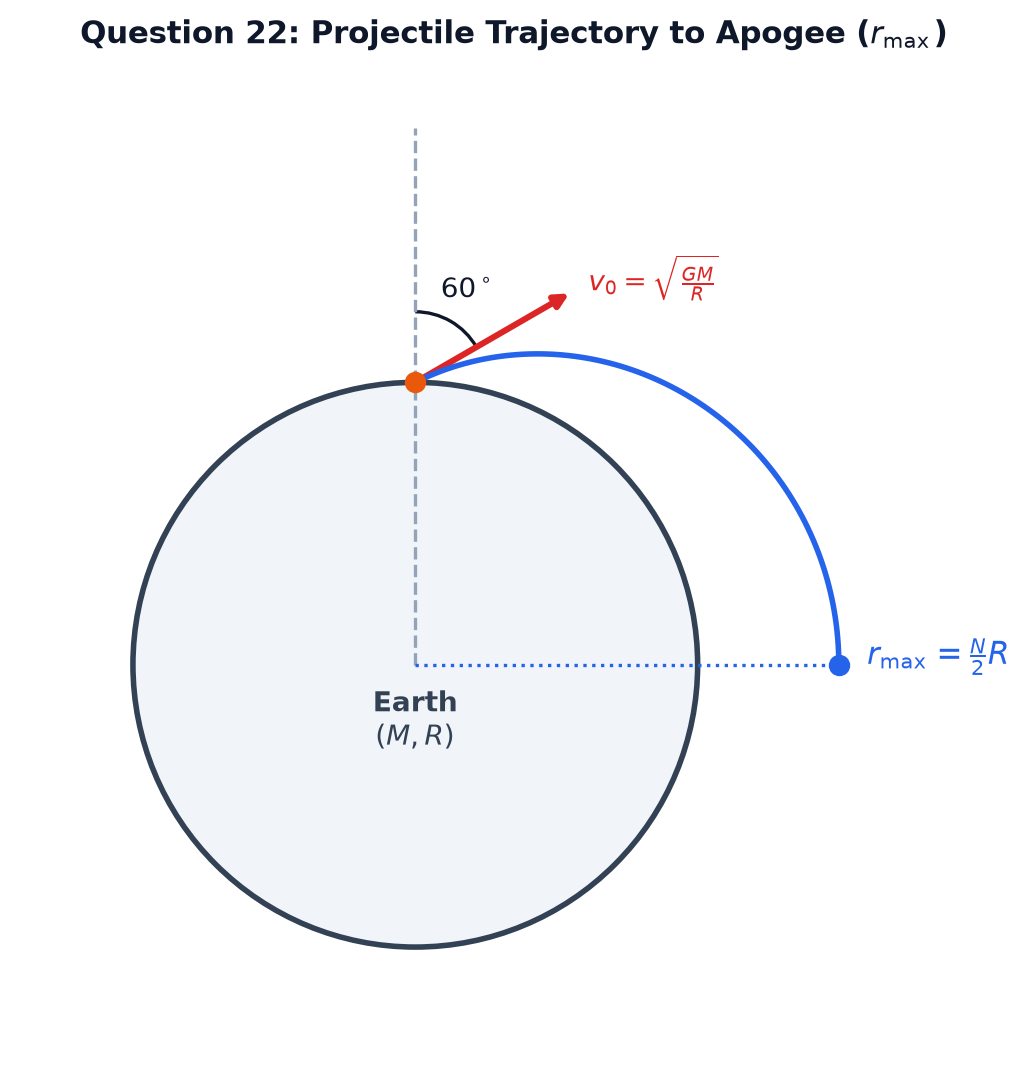
\includegraphics[width=0.34\textwidth]{images/sohan_grav_q22_projectile.png}
  \end{center}

  \item A satellite is initially in a circular orbit of radius $r_1 = 2R$ around Earth. It is transferred to a higher circular orbit of radius $r_2 = 6R$ using a semi-elliptical Hohmann transfer orbit, as illustrated in the figure. If $T_0$ is the orbital period of a hypothetical satellite orbiting Earth at surface radius $R$, the transfer time from orbit 1 to orbit 2 is $t_{\text{transfer}} = k T_0$. Find the integer value of $k$.
  \begin{center}
    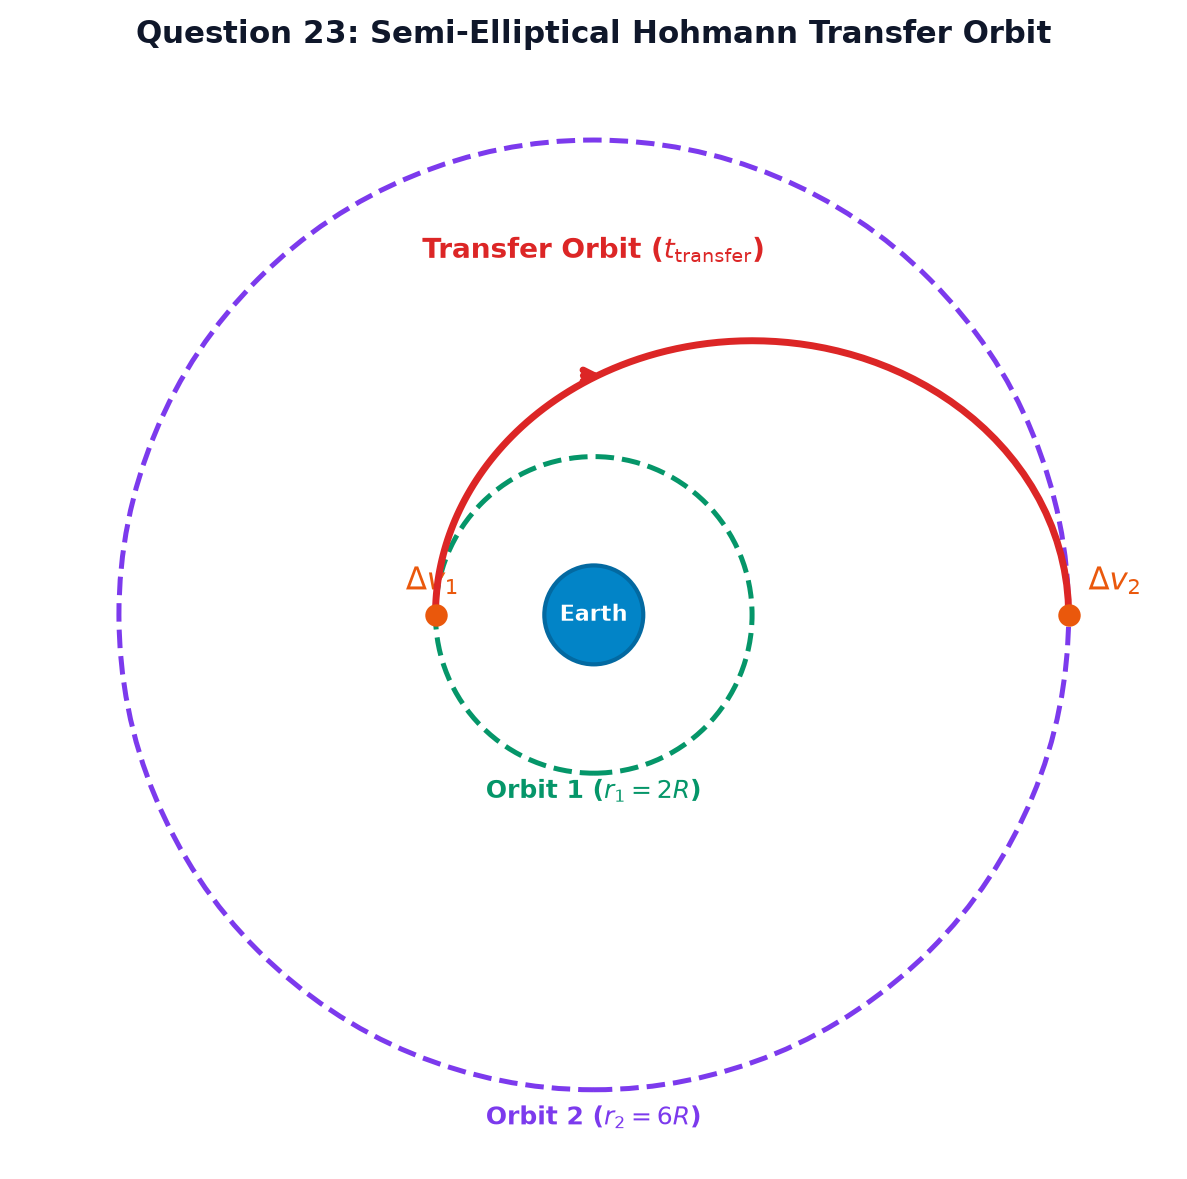
\includegraphics[width=0.38\textwidth]{images/sohan_grav_q23_hohmann.png}
  \end{center}

  \item A particle of mass $m$ is at the center of a uniform solid sphere of mass $M$ and radius $R$. The ratio of the escape speed required to send this particle from the center to infinity to the escape speed from the surface of the sphere is $\sqrt{\dfrac{k}{2}}$. Find the integer value of $k$.

  \item Three identical stars, each of mass $M$, move in circular orbits around their common center of mass under mutual gravitational attraction, always maintaining an equilateral triangle of side $a$. If the side of the equilateral triangle is increased to $2a$, the ratio of the original orbital speed to the new orbital speed is $\sqrt{N}$. Find the integer value of $N$.

\end{enumerate}

\newpage

% ==================== MASTER ANSWER KEY ====================
\begin{tcolorbox}[sectionbanner]
  {\large \textbf{\textsf{MASTER 100\% VERIFIED ANSWER KEY}}}
\end{tcolorbox}
\vspace{4pt}

\begin{center}
\renewcommand{\arraystretch}{1.25}
\small
\begin{tabularx}{\textwidth}{|>{\centering\arraybackslash}c|>{\centering\arraybackslash}c|>{\centering\arraybackslash}c|>{\centering\arraybackslash}c|>{\centering\arraybackslash}c|>{\centering\arraybackslash}c|>{\centering\arraybackslash}c|>{\centering\arraybackslash}c|>{\centering\arraybackslash}c|>{\centering\arraybackslash}X|}
\hline
\rowcolor{tableDarkHeader}
\textcolor{white}{\textbf{Q.}} & \textcolor{white}{\textbf{Ans}} & \textcolor{white}{\textbf{Q.}} & \textcolor{white}{\textbf{Ans}} & \textcolor{white}{\textbf{Q.}} & \textcolor{white}{\textbf{Ans}} & \textcolor{white}{\textbf{Q.}} & \textcolor{white}{\textbf{Ans}} & \textcolor{white}{\textbf{Q.}} & \textcolor{white}{\textbf{Ans}} \\
\hline
\rowcolor{white}
\textbf{01} & B & \textbf{06} & B & \textbf{11} & A & \textbf{16} & A & \textbf{21} & \textbf{2} \\
\hline
\rowcolor{tableStripe}
\textbf{02} & C & \textbf{07} & B & \textbf{12} & C & \textbf{17} & A & \textbf{22} & \textbf{3} \\
\hline
\rowcolor{white}
\textbf{03} & C & \textbf{08} & A & \textbf{13} & A & \textbf{18} & A & \textbf{23} & \textbf{4} \\
\hline
\rowcolor{tableStripe}
\textbf{04} & A & \textbf{09} & B & \textbf{14} & B & \textbf{19} & A & \textbf{24} & \textbf{3} \\
\hline
\rowcolor{white}
\textbf{05} & A & \textbf{10} & A & \textbf{15} & C & \textbf{20} & A & \textbf{25} & \textbf{2} \\
\hline
\end{tabularx}
\end{center}

\vspace{10pt}

% ==================== COMPREHENSIVE SOLUTIONS ====================
\begin{tcolorbox}[sectionbanner]
  {\large \textbf{\textsf{COMPREHENSIVE STEP-BY-STEP SOLUTIONS}}}
\end{tcolorbox}
\vspace{4pt}

\begin{tcolorbox}[solbox]
  \textbf{\textcolor{primaryDark}{Question 1:}} \hfill \textbf{\textcolor{l3Crimson}{Answer: B}}\\
  \vspace{3pt}
  By conservation of angular momentum about the center of Earth:
$$v_p r_p = v_a r_a \implies v_a = v_p \frac{r_p}{r_a} = v_p \frac{2R}{6R} = \frac{1}{3}v_p$$
\vspace{3pt}
By conservation of mechanical energy:
$$\frac{1}{2}m v_p^2 - \frac{GMm}{r_p} = \frac{1}{2}m v_a^2 - \frac{GMm}{r_a}$$
$$\frac{1}{2}v_p^2 - \frac{GM}{2R} = \frac{1}{2}\left(\frac{v_p}{3}\right)^2 - \frac{GM}{6R}$$
$$\frac{1}{2}v_p^2 \left(1 - \frac{1}{9}\right) = \frac{GM}{R}\left(\frac{1}{2} - \frac{1}{6}\right) = \frac{GM}{3R}$$
$$\frac{4}{9}v_p^2 = \frac{GM}{3R} \implies v_p^2 = \frac{3GM}{4R} \implies v_p = \frac{\sqrt{3}}{2}\sqrt{\frac{GM}{R}}$$
\vspace{3pt}
Hence, the correct option is \textbf{(B)}\textbf{.}
\end{tcolorbox}
\vspace{3pt}

\begin{tcolorbox}[solbox]
  \textbf{\textcolor{primaryDark}{Question 2:}} \hfill \textbf{\textcolor{l3Crimson}{Answer: C}}\\
  \vspace{3pt}
  By the principle of superposition, the sphere with a cavity is equivalent to a complete solid sphere of density $+\rho$ plus a sphere of radius $R/2$ and density $-\rho$ centered at $\vec{d}$.
\vspace{3pt}
For any point inside the cavity with position vector $\vec{r}$ relative to the sphere's center, its position vector relative to the cavity's center is $\vec{r}' = \vec{r} - \vec{d}$.
\vspace{3pt}
The field due to the entire solid sphere is:
$$\vec{g}_1 = -\frac{4}{3}\pi G \rho \vec{r}$$
The field due to the removed cavity mass (negative mass) is:
$$\vec{g}_2 = +\frac{4}{3}\pi G \rho (\vec{r} - \vec{d})$$
\vspace{3pt}
Total gravitational field inside the cavity:
$$\vec{g} = \vec{g}_1 + \vec{g}_2 = -\frac{4}{3}\pi G \rho \vec{r} + \frac{4}{3}\pi G \rho (\vec{r} - \vec{d}) = -\frac{4}{3}\pi G \rho \vec{d}$$
\vspace{3pt}
Magnitude: $|\vec{g}| = \frac{4}{3}\pi G \rho |\vec{d}| = \frac{4}{3}\pi G \rho \left(\frac{R}{2}\right) = \frac{2}{3}\pi G \rho R$.
The field is completely uniform in magnitude and directed strictly opposite to $\vec{d}$.
\vspace{3pt}
Hence, the correct option is \textbf{(C)}\textbf{.}
\end{tcolorbox}
\vspace{3pt}

\begin{tcolorbox}[solbox]
  \textbf{\textcolor{primaryDark}{Question 3:}} \hfill \textbf{\textcolor{l3Crimson}{Answer: C}}\\
  \vspace{3pt}
  At a displacement $x$ along the tunnel from its midpoint, the distance of the particle from the center of Earth is $r = \sqrt{x^2 + d^2}$.
\vspace{3pt}
The gravitational field inside Earth is:
$$\vec{g}(r) = -\frac{g}{R}\vec{r} = -\frac{g}{R}(x\hat{i} + d\hat{j})$$
\vspace{3pt}
1. Along the tunnel ($\hat{i}$):
$$F_x = -m\frac{g}{R}x = -m\omega^2 x$$
This is the defining equation of simple harmonic motion with $\omega = \sqrt{g/R}$ and period $T = 2\pi\sqrt{R/g}$. Statements (A) and (B) are true.
\vspace{3pt}
2. Perpendicular to the tunnel ($\hat{j}$):
The normal reaction force $N$ balances the perpendicular component of gravity:
$$N = m\frac{g}{R}d = m\frac{g}{R}\left(\frac{R}{2}\right) = \frac{mg}{2}$$
Notice that $N$ is completely independent of $x$ and time $t$! Statement (D) is true, which makes statement (C) incorrect.
\vspace{3pt}
Hence, the correct option is \textbf{(C)}\textbf{.}
\end{tcolorbox}
\vspace{3pt}

\begin{tcolorbox}[solbox]
  \textbf{\textcolor{primaryDark}{Question 4:}} \hfill \textbf{\textcolor{l3Crimson}{Answer: A}}\\
  \vspace{3pt}
  At the grazing threshold, the closest distance from the center is $r_{\min} = R$, where the velocity vector is perpendicular to the radial vector ($v = v_{\max}$).
\vspace{3pt}
By conservation of angular momentum about the planet's center:
$$m v_0 b = m v_{\max} R \implies v_{\max} = v_0 \frac{b}{R}$$
\vspace{3pt}
By conservation of mechanical energy:
$$\frac{1}{2}m v_0^2 + 0 = \frac{1}{2}m v_{\max}^2 - \frac{GMm}{R}$$
$$\frac{1}{2}v_0^2 = \frac{1}{2}v_0^2\left(\frac{b}{R}\right)^2 - \frac{GM}{R}$$
$$\frac{b^2}{R^2} = 1 + \frac{2GM}{R v_0^2} \implies b \le R\sqrt{1 + \frac{2GM}{R v_0^2}}$$
\vspace{3pt}
Hence, the correct option is \textbf{(A)}\textbf{.}
\end{tcolorbox}
\vspace{3pt}

\begin{tcolorbox}[solbox]
  \textbf{\textcolor{primaryDark}{Question 5:}} \hfill \textbf{\textcolor{l3Crimson}{Answer: A}}\\
  \vspace{3pt}
  In an equilateral triangle inscribed in a circle of radius $R$, the side length is $a = 2R\cos 30^\circ = R\sqrt{3}$.
\vspace{3pt}
The gravitational attraction on any one star due to each of the other two stars is:
$$F = \frac{GM^2}{a^2} = \frac{GM^2}{3R^2}$$
The angle between these two force vectors is $60^\circ$. The resultant inward force directed towards the centroid is:
$$F_{\text{net}} = 2 F \cos 30^\circ = 2\left(\frac{GM^2}{3R^2}\right)\frac{\sqrt{3}}{2} = \frac{GM^2}{R^2\sqrt{3}}$$
\vspace{3pt}
Equating to centripetal force $\frac{M v^2}{R}$:
$$\frac{M v^2}{R} = \frac{GM^2}{R^2\sqrt{3}} \implies v = \sqrt{\frac{GM}{R\sqrt{3}}}$$
\vspace{3pt}
The orbital period is:
$$T = \frac{2\pi R}{v} = 2\pi R \sqrt{\frac{R\sqrt{3}}{GM}} = 2\pi \sqrt{\frac{R^3\sqrt{3}}{GM}}$$
\vspace{3pt}
Hence, the correct option is \textbf{(A)}\textbf{.}
\end{tcolorbox}
\vspace{3pt}

\begin{tcolorbox}[solbox]
  \textbf{\textcolor{primaryDark}{Question 6:}} \hfill \textbf{\textcolor{l3Crimson}{Answer: B}}\\
  \vspace{3pt}
  The mass enclosed inside a concentric sphere of radius $r$ ($r \le R$) is:
$$M(r) = \int_0^r 4\pi x^2 \rho(x)\,dx = 4\pi\rho_0 \int_0^r \left(x^2 - \frac{x^3}{R}\right)dx = 4\pi\rho_0 \left[\frac{r^3}{3} - \frac{r^4}{4R}\right]$$
\vspace{3pt}
By Newton's shell theorem, the gravitational field intensity at radius $r$ is:
$$g(r) = \frac{G M(r)}{r^2} = 4\pi G \rho_0 \left[\frac{r}{3} - \frac{r^2}{4R}\right]$$
\vspace{3pt}
To find the radius of maximum field, differentiate $g(r)$ with respect to $r$ and set to zero:
$$\frac{dg}{dr} = 4\pi G \rho_0 \left[\frac{1}{3} - \frac{2r}{4R}\right] = 0$$
$$\frac{1}{3} - \frac{r}{2R} = 0 \implies r = \frac{2R}{3}$$
\vspace{3pt}
Hence, the correct option is \textbf{(B)}\textbf{.}
\end{tcolorbox}
\vspace{3pt}

\begin{tcolorbox}[solbox]
  \textbf{\textcolor{primaryDark}{Question 7:}} \hfill \textbf{\textcolor{l3Crimson}{Answer: B}}\\
  \vspace{3pt}
  The gravitational potential at the center of a uniform solid sphere of mass $M$ and radius $R$ is:
$$V(0) = -\frac{3GM}{2R}$$
\vspace{3pt}
To escape to infinity where $V(\infty) = 0$, the total mechanical energy must be non-negative:
$$E = \frac{1}{2}m v^2 + m V(0) \ge 0 \implies \frac{1}{2}m v^2 - \frac{3GMm}{2R} \ge 0$$
$$v \ge \sqrt{\frac{3GM}{R}}$$
\vspace{3pt}
Since escape velocity from the surface is $v_e = \sqrt{\frac{2GM}{R}}$:
$$v = \sqrt{\frac{3}{2}}\sqrt{\frac{2GM}{R}} = \sqrt{1.5}\,v_e$$
\vspace{3pt}
Hence, the correct option is \textbf{(B)}\textbf{.}
\end{tcolorbox}
\vspace{3pt}

\begin{tcolorbox}[solbox]
  \textbf{\textcolor{primaryDark}{Question 8:}} \hfill \textbf{\textcolor{l3Crimson}{Answer: A}}\\
  \vspace{3pt}
  Initial circular orbital speed at $r_1 = R$:
$$v_c = \sqrt{\frac{GM}{R}}$$
\vspace{3pt}
The transfer elliptical orbit has major axis $2a = r_1 + r_2 = R + 4R = 5R \implies a = \frac{5}{2}R$.
Using the vis-viva equation $v^2 = GM\left(\frac{2}{r} - \frac{1}{a}\right)$, the velocity at the perigee ($r = R$) of the transfer ellipse is:
$$v_1^2 = GM\left(\frac{2}{R} - \frac{1}{\frac{5}{2}R}\right) = GM\left(\frac{2}{R} - \frac{2}{5R}\right) = \frac{8GM}{5R}$$
$$v_1 = \sqrt{\frac{8GM}{5R}}$$
\vspace{3pt}
The velocity boost $\Delta v_1$ required is:
$$\Delta v_1 = v_1 - v_c = \sqrt{\frac{8GM}{5R}} - \sqrt{\frac{GM}{R}} = \left(\sqrt{\frac{8}{5}} - 1\right)\sqrt{\frac{GM}{R}}$$
\vspace{3pt}
Hence, the correct option is \textbf{(A)}\textbf{.}
\end{tcolorbox}
\vspace{3pt}

\begin{tcolorbox}[solbox]
  \textbf{\textcolor{primaryDark}{Question 9:}} \hfill \textbf{\textcolor{l3Crimson}{Answer: B}}\\
  \vspace{3pt}
  The binding energy of the spherical planet is defined as the work required to dismantle it and transport all its mass elements to infinity against their mutual gravitational attraction:
$$W_{\text{ext}} = U_{\infty} - U_{\text{initial}} = 0 - \left(-\frac{3GM^2}{5R}\right) = \frac{3GM^2}{5R}$$
\vspace{3pt}
Hence, the correct option is \textbf{(B)}\textbf{.}
\end{tcolorbox}
\vspace{3pt}

\begin{tcolorbox}[solbox]
  \textbf{\textcolor{primaryDark}{Question 10:}} \hfill \textbf{\textcolor{l3Crimson}{Answer: A}}\\
  \vspace{3pt}
  Consider a thin elemental ring on the hemispherical shell at angular elevation $\theta$ from the $z$-axis of symmetry (where $0 \le \theta \le \pi/2$):
Area of the hemisphere $= 2\pi R^2$.
Area of elemental ring $= 2\pi (R\sin\theta)(R\,d\theta) = 2\pi R^2\sin\theta\,d\theta$.
Mass of the elemental ring: $dm = M\sin\theta\,d\theta$.
\vspace{3pt}
Every point on this ring is at a distance $R$ from the center $O$. By symmetry, horizontal components cancel, and the vertical field component along $z$ is:
$$dg_z = \frac{G\,dm}{R^2}\cos\theta = \frac{GM}{R^2}\sin\theta\cos\theta\,d\theta$$
\vspace{3pt}
Integrating from $\theta = 0$ to $\pi/2$:
$$g = \frac{GM}{R^2}\int_0^{\pi/2}\sin\theta\cos\theta\,d\theta = \frac{GM}{R^2}\left[\frac{\sin^2\theta}{2}\right]_0^{\pi/2} = \frac{GM}{2R^2}$$
\vspace{3pt}
Hence, the correct option is \textbf{(A)}\textbf{.}
\end{tcolorbox}
\vspace{3pt}

\begin{tcolorbox}[solbox]
  \textbf{\textcolor{primaryDark}{Question 11:}} \hfill \textbf{\textcolor{l3Crimson}{Answer: A}}\\
  \vspace{3pt}
  The axial gravitational field of a ring of mass $M$ and radius $R$ is:
$$g(x) = \frac{GMx}{(R^2 + x^2)^{3/2}}$$
\vspace{3pt}
To find the maximum, set $\frac{dg}{dx} = 0$:
$$\frac{d}{dx}\left[\frac{x}{(R^2 + x^2)^{3/2}}\right] = \frac{(R^2 + x^2)^{3/2} - x\left(\frac{3}{2}\right)(R^2 + x^2)^{1/2}(2x)}{(R^2 + x^2)^3} = 0$$
$$(R^2 + x^2) - 3x^2 = 0 \implies R^2 = 2x^2 \implies x = \frac{R}{\sqrt{2}}$$
\vspace{3pt}
Substituting $x = \frac{R}{\sqrt{2}}$ into $g(x)$:
$$g_{\max} = \frac{GM(R/\sqrt{2})}{(R^2 + R^2/2)^{3/2}} = \frac{GM R/\sqrt{2}}{\left(\frac{3}{2}R^2\right)^{3/2}} = \frac{GM R/\sqrt{2}}{\frac{3\sqrt{3}}{2\sqrt{2}}R^3} = \frac{2GM}{3\sqrt{3}R^2}$$
\vspace{3pt}
Hence, the correct option is \textbf{(A)}\textbf{.}
\end{tcolorbox}
\vspace{3pt}

\begin{tcolorbox}[solbox]
  \textbf{\textcolor{primaryDark}{Question 12:}} \hfill \textbf{\textcolor{l3Crimson}{Answer: C}}\\
  \vspace{3pt}
  In the rotating reference frame of Earth, two forces act on a mass $m$ at latitude $\lambda$:
1. True gravitational force directed radially inward: $F_g = mg$.
2. Centrifugal force directed perpendicular to the rotation axis outward: $F_{cf} = m\omega^2 R\cos\lambda$.
\vspace{3pt}
Resolving forces along and perpendicular to the local vertical:
Tangential component towards the equator:
$$F_t = F_{cf}\sin\lambda = m\omega^2 R\cos\lambda\sin\lambda = \frac{1}{2}m\omega^2 R\sin(2\lambda)$$
Radial component inwards:
$$F_r \approx mg$$
\vspace{3pt}
The deflection angle $\alpha$ of the plumb line from the true radial line is:
$$\tan\alpha \approx \frac{F_t}{F_r} = \frac{\omega^2 R\sin(2\lambda)}{2g}$$
This angle is maximum when $\sin(2\lambda)$ is maximum ($= 1$), which occurs at $2\lambda = 90^\circ \implies \lambda = 45^\circ$.
\vspace{3pt}
Hence, the correct option is \textbf{(C)}\textbf{.}
\end{tcolorbox}
\vspace{3pt}

\begin{tcolorbox}[solbox]
  \textbf{\textcolor{primaryDark}{Question 13:}} \hfill \textbf{\textcolor{l3Crimson}{Answer: A}}\\
  \vspace{3pt}
  Since no external forces act on the two-body system, the center of mass remains at rest:
$$M \Delta x_1 = 5M \Delta x_2 \implies \Delta x_1 = 5 \Delta x_2$$
\vspace{3pt}
Initially, center-to-center distance is $d_i = 12R$.
At the instant of collision (physical contact), the center-to-center distance is:
$$d_f = R + 2R = 3R$$
Total reduction in center-to-center distance:
$$\Delta x_1 + \Delta x_2 = d_i - d_f = 12R - 3R = 9R$$
\vspace{3pt}
Substituting $\Delta x_1 = 5\Delta x_2$:
$$5\Delta x_2 + \Delta x_2 = 9R \implies 6\Delta x_2 = 9R \implies \Delta x_2 = 1.5R$$
Therefore, distance traveled by mass $M$ is:
$$\Delta x_1 = 5(1.5R) = 7.5R$$
\vspace{3pt}
Hence, the correct option is \textbf{(A)}\textbf{.}
\end{tcolorbox}
\vspace{3pt}

\begin{tcolorbox}[solbox]
  \textbf{\textcolor{primaryDark}{Question 14:}} \hfill \textbf{\textcolor{l3Crimson}{Answer: B}}\\
  \vspace{3pt}
  By conservation of mechanical energy:
$$E_i = \frac{1}{2}m v^2 - \frac{GMm}{R}$$
Since $v_e^2 = \frac{2GM}{R} \implies \frac{GMm}{R} = \frac{1}{2}m v_e^2$:
$$E_i = \frac{1}{2}m v^2 - \frac{1}{2}m v_e^2$$
\vspace{3pt}
At infinity, gravitational potential energy is zero, so $E_f = \frac{1}{2}m v_\infty^2$.
Equating energies:
$$\frac{1}{2}m v_\infty^2 = \frac{1}{2}m(v^2 - v_e^2) \implies v_\infty = \sqrt{v^2 - v_e^2}$$
\vspace{3pt}
Given $v = \sqrt{5}\,v_e$:
$$v_\infty = \sqrt{(\sqrt{5}\,v_e)^2 - v_e^2} = \sqrt{5v_e^2 - v_e^2} = \sqrt{4v_e^2} = 2v_e$$
\vspace{3pt}
Hence, the correct option is \textbf{(B)}\textbf{.}
\end{tcolorbox}
\vspace{3pt}

\begin{tcolorbox}[solbox]
  \textbf{\textcolor{primaryDark}{Question 15:}} \hfill \textbf{\textcolor{l3Crimson}{Answer: C}}\\
  \vspace{3pt}
  For a circular orbit grazing the planet's surface ($r \approx R$):
$$v = \sqrt{\frac{GM}{R}}$$
Orbital period:
$$T = \frac{2\pi R}{v} = \frac{2\pi R}{\sqrt{GM/R}} = 2\pi \sqrt{\frac{R^3}{GM}}$$
\vspace{3pt}
Expressing mass in terms of uniform density $\rho$:
$$M = \frac{4}{3}\pi R^3 \rho$$
$$T = 2\pi \sqrt{\frac{R^3}{G\left(\frac{4}{3}\pi R^3 \rho\right)}} = 2\pi \sqrt{\frac{3}{4\pi G \rho}} = \sqrt{\frac{3\pi}{G\rho}}$$
\vspace{3pt}
Notice that the radius $R$ cancels completely! The orbital period depends strictly on the mean density $\rho$ of the planet.
\vspace{3pt}
Hence, the correct option is \textbf{(C)}\textbf{.}
\end{tcolorbox}
\vspace{3pt}

\begin{tcolorbox}[solbox]
  \textbf{\textcolor{primaryDark}{Question 16:}} \hfill \textbf{\textcolor{l3Crimson}{Answer: A}}\\
  \vspace{3pt}
  Gravitational potential at the surface of the inner shell ($r = R_1$):
$$V(R_1) = -\frac{GM_1}{R_1} - \frac{GM_2}{R_2}$$
\vspace{3pt}
Gravitational potential at the surface of the outer shell ($r = R_2$):
$$V(R_2) = -\frac{GM_1}{R_2} - \frac{GM_2}{R_2}$$
\vspace{3pt}
Work done by external agent in moving mass $m$ slowly:
$$W_{\text{ext}} = m [V(R_2) - V(R_1)] = m \left[\left(-\frac{GM_1}{R_2} - \frac{GM_2}{R_2}\right) - \left(-\frac{GM_1}{R_1} - \frac{GM_2}{R_2}\right)\right]$$
$$W_{\text{ext}} = GM_1 m \left(\frac{1}{R_1} - \frac{1}{R_2}\right)$$
\vspace{3pt}
The contribution from $M_2$ cancels out identically because potential inside a spherical shell is constant.
\vspace{3pt}
Hence, the correct option is \textbf{(A)}\textbf{.}
\end{tcolorbox}
\vspace{3pt}

\begin{tcolorbox}[solbox]
  \textbf{\textcolor{primaryDark}{Question 17:}} \hfill \textbf{\textcolor{l3Crimson}{Answer: A}}\\
  \vspace{3pt}
  In an elliptical orbit with semi-major axis $a$ and eccentricity $e$:
Perihelion distance: $r_p = a(1 - e)$
Aphelion distance: $r_a = a(1 + e)$
\vspace{3pt}
By conservation of angular momentum about the focus:
$$L = m v_p r_p = m v_a r_a \implies \frac{v_p}{v_a} = \frac{r_a}{r_p} = \frac{a(1 + e)}{a(1 - e)} = \frac{1 + e}{1 - e}$$
\vspace{3pt}
Hence, the correct option is \textbf{(A)}\textbf{.}
\end{tcolorbox}
\vspace{3pt}

\begin{tcolorbox}[solbox]
  \textbf{\textcolor{primaryDark}{Question 18:}} \hfill \textbf{\textcolor{l3Crimson}{Answer: A}}\\
  \vspace{3pt}
  The two masses are at radial positions $r_1 = r - \ell$ and $r_2 = r + \ell$.
The difference in gravitational forces exerted on them is:
$$\Delta F = \frac{GMm}{(r-\ell)^2} - \frac{GMm}{(r+\ell)^2} = \frac{GMm}{r^2}\left[\left(1 - \frac{\ell}{r}\right)^{-2} - \left(1 + \frac{\ell}{r}\right)^{-2}\right]$$
Using binomial expansion for $\ell \ll r$:
$$\Delta F \approx \frac{GMm}{r^2}\left[\left(1 + \frac{2\ell}{r}\right) - \left(1 - \frac{2\ell}{r}\right)\right] = \frac{GMm}{r^2}\left(\frac{4\ell}{r}\right) = \frac{4GMm\ell}{r^3}$$
\vspace{3pt}
Relative to the center of mass of the dumbbell, each mass experiences a differential tidal pull of:
$$F_{\text{tide}} = \frac{1}{2}\Delta F = \frac{2GMm\ell}{r^3}$$
\vspace{3pt}
Hence, the correct option is \textbf{(A)}\textbf{.}
\end{tcolorbox}
\vspace{3pt}

\begin{tcolorbox}[solbox]
  \textbf{\textcolor{primaryDark}{Question 19:}} \hfill \textbf{\textcolor{l3Crimson}{Answer: A}}\\
  \vspace{3pt}
  The mass enclosed inside a sphere of radius $r$ is:
$$M(r) = \int_0^r 4\pi x^2 \rho(x)\,dx = \int_0^r 4\pi x^2 \left(\frac{C}{x}\right)dx = 4\pi C \int_0^r x\,dx = 2\pi C r^2$$
\vspace{3pt}
By Newton's shell theorem, the gravitational field intensity at radius $r$ is:
$$g(r) = \frac{G M(r)}{r^2} = \frac{G(2\pi C r^2)}{r^2} = 2\pi G C$$
\vspace{3pt}
Notice that $r$ cancels out completely! The gravitational field intensity inside this cloud is strictly uniform and constant throughout.
\vspace{3pt}
Hence, the correct option is \textbf{(A)}\textbf{.}
\end{tcolorbox}
\vspace{3pt}

\begin{tcolorbox}[solbox]
  \textbf{\textcolor{primaryDark}{Question 20:}} \hfill \textbf{\textcolor{l3Crimson}{Answer: A}}\\
  \vspace{3pt}
  By Newton's spherical shell theorem, the external gravitational field produced by a uniform solid sphere of mass $M$ is identical to that of a point mass $M$ situated at its center $O$.
\vspace{3pt}
The ring of mass $m$ and radius $R$ lies in a horizontal plane at vertical distance $h = R$ along its axis from point $O$.
The gravitational force exerted by a ring of mass $m$ on a point mass $M$ along its axis at distance $h$ is:
$$F = \frac{GMmh}{(R^2 + h^2)^{3/2}}$$
\vspace{3pt}
Substituting $h = R$:
$$F = \frac{GMm R}{(R^2 + R^2)^{3/2}} = \frac{GMm R}{(2R^2)^{3/2}} = \frac{GMm R}{2\sqrt{2}R^3} = \frac{GMm}{2\sqrt{2}R^2}$$
\vspace{3pt}
Hence, the correct option is \textbf{(A)}\textbf{.}
\end{tcolorbox}
\vspace{3pt}

\begin{tcolorbox}[solbox]
  \textbf{\textcolor{primaryDark}{Question 21:}} \hfill \textbf{\textcolor{l3Crimson}{Answer: 2}}\\
  \vspace{3pt}
  Initial position: $r_i = R + h = 2R$.
Initial mechanical energy of the body:
$$E_i = K_i + U_i = 0 - \frac{GMm}{2R} = -\frac{GMm}{2R}$$
\vspace{3pt}
At the center of Earth ($r = 0$), the gravitational potential is:
$$V(0) = -\frac{3GM}{2R}$$
Final mechanical energy:
$$E_f = \frac{1}{2}m v^2 + m V(0) = \frac{1}{2}m v^2 - \frac{3GMm}{2R}$$
\vspace{3pt}
By conservation of mechanical energy ($E_i = E_f$):
$$-\frac{GMm}{2R} = \frac{1}{2}m v^2 - \frac{3GMm}{2R}$$
$$\frac{1}{2}m v^2 = \frac{3GMm}{2R} - \frac{GMm}{2R} = \frac{GMm}{R}$$
$$v^2 = \frac{2GM}{R} = 2gR \implies v = \sqrt{2gR}$$
\vspace{3pt}
Comparing with $v = \sqrt{\alpha g R}$, we obtain $\alpha = 2$.
\end{tcolorbox}
\vspace{3pt}

\begin{tcolorbox}[solbox]
  \textbf{\textcolor{primaryDark}{Question 22:}} \hfill \textbf{\textcolor{l3Crimson}{Answer: 3}}\\
  \vspace{3pt}
  At launch ($r = R$):
Speed $v_0 = \sqrt{\frac{GM}{R}}$.
Angle with vertical is $60^\circ$, so the tangential velocity is:
$$v_{0\perp} = v_0\sin 60^\circ = \frac{\sqrt{3}}{2}\sqrt{\frac{GM}{R}}$$
\vspace{3pt}
At the apogee ($r_{\max}$), velocity is purely tangential ($v = v_{\text{apo}}$).
Conservation of angular momentum about Earth's center:
$$R v_{0\perp} = r_{\max} v_{\text{apo}} \implies v_{\text{apo}} = \frac{R}{r_{\max}}\left(\frac{\sqrt{3}}{2}\sqrt{\frac{GM}{R}}\right)$$
\vspace{3pt}
Conservation of mechanical energy:
$$\frac{1}{2}v_0^2 - \frac{GM}{R} = \frac{1}{2}v_{\text{apo}}^2 - \frac{GM}{r_{\max}}$$
$$\frac{1}{2}\frac{GM}{R} - \frac{GM}{R} = \frac{1}{2}\frac{3GMR}{4 r_{\max}^2} - \frac{GM}{r_{\max}}$$
$$-\frac{1}{2R} = \frac{3R}{8 r_{\max}^2} - \frac{1}{r_{\max}}$$
\vspace{3pt}
Multiplying both sides by $8R r_{\max}^2$:
$$-4 r_{\max}^2 = 3R^2 - 8R r_{\max} \implies 4 r_{\max}^2 - 8R r_{\max} + 3R^2 = 0$$
$$(2r_{\max} - R)(2r_{\max} - 3R) = 0$$
Since $r_{\max} > R$:
$$2r_{\max} = 3R \implies r_{\max} = \frac{3}{2}R$$
\vspace{3pt}
Comparing with $r_{\max} = \frac{N}{2}R$, we find $N = 3$.
\end{tcolorbox}
\vspace{3pt}

\begin{tcolorbox}[solbox]
  \textbf{\textcolor{primaryDark}{Question 23:}} \hfill \textbf{\textcolor{l3Crimson}{Answer: 4}}\\
  \vspace{3pt}
  The semi-major axis of the elliptical Hohmann transfer orbit is:
$$a = \frac{r_1 + r_2}{2} = \frac{2R + 6R}{2} = 4R$$
\vspace{3pt}
By Kepler's Third Law ($T^2 \propto a^3$):
$$\frac{T_{\text{ellipse}}}{T_0} = \left(\frac{a}{R}\right)^{3/2} = (4)^{3/2} = 8 \implies T_{\text{ellipse}} = 8 T_0$$
\vspace{3pt}
The transfer time is half of the orbital period of the ellipse (from perigee to apogee):
$$t_{\text{transfer}} = \frac{1}{2} T_{\text{ellipse}} = \frac{1}{2}(8 T_0) = 4 T_0$$
\vspace{3pt}
Comparing with $t_{\text{transfer}} = k T_0$, we obtain $k = 4$.
\end{tcolorbox}
\vspace{3pt}

\begin{tcolorbox}[solbox]
  \textbf{\textcolor{primaryDark}{Question 24:}} \hfill \textbf{\textcolor{l3Crimson}{Answer: 3}}\\
  \vspace{3pt}
  1. Escape speed from surface:
$$v_{\text{surf}} = \sqrt{\frac{2GM}{R}}$$
\vspace{3pt}
2. Escape speed from center:
Potential at center: $V(0) = -\frac{3GM}{2R}$.
Energy required to escape:
$$\frac{1}{2}m v_{\text{center}}^2 + m V(0) = 0 \implies v_{\text{center}} = \sqrt{\frac{3GM}{R}}$$
\vspace{3pt}
Ratio:
$$\frac{v_{\text{center}}}{v_{\text{surf}}} = \frac{\sqrt{3GM/R}}{\sqrt{2GM/R}} = \sqrt{\frac{3}{2}}$$
\vspace{3pt}
Comparing with $\sqrt{\frac{k}{2}}$, we find $k = 3$.
\end{tcolorbox}
\vspace{3pt}

\begin{tcolorbox}[solbox]
  \textbf{\textcolor{primaryDark}{Question 25:}} \hfill \textbf{\textcolor{l3Crimson}{Answer: 2}}\\
  \vspace{3pt}
  For three equal stars of mass $M$ at the vertices of an equilateral triangle of side $a$, the orbital radius about the centroid is $R = \frac{a}{\sqrt{3}}$.
\vspace{3pt}
The net gravitational force towards the centroid on each star is:
$$F_{\text{net}} = 2\left(\frac{GM^2}{a^2}\right)\cos 30^\circ = \sqrt{3}\frac{GM^2}{a^2}$$
Equating to centripetal force:
$$\frac{M v^2}{R} = \frac{M v^2}{a/\sqrt{3}} = \sqrt{3}\frac{M v^2}{a} = \sqrt{3}\frac{GM^2}{a^2} \implies v = \sqrt{\frac{GM}{a}}$$
\vspace{3pt}
Therefore, orbital speed scales as:
$$v \propto \frac{1}{\sqrt{a}}$$
When the side length is doubled ($a' = 2a$):
$$\frac{v}{v'} = \sqrt{\frac{a'}{a}} = \sqrt{\frac{2a}{a}} = \sqrt{2}$$
\vspace{3pt}
Comparing with $\sqrt{N}$, we find $N = 2$.
\end{tcolorbox}
\vspace{3pt}

\end{document}
